% !TEX root = ../../../main.tex
% 来源：中学数学实验教材·第三册（高中数学）
% 章节：函数及其图象 / 一次函数（线性函数）
% 原始文件：4.tex，行 2637-2654
% 类型：tikz
% ---
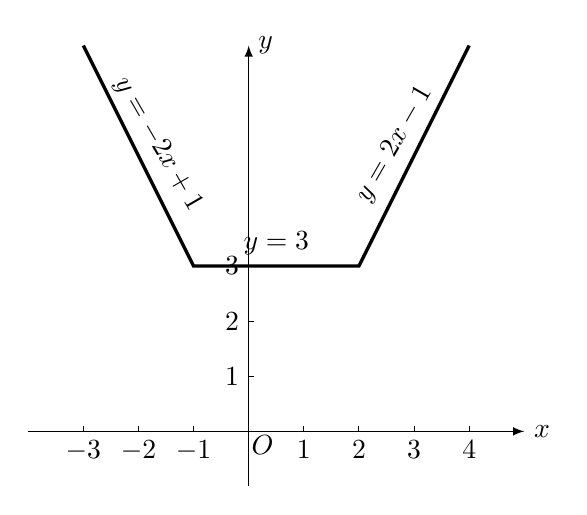
\begin{tikzpicture}[>=latex, scale=.7]
    \draw[->] (-4,0) --(5,0)node[right]{$x$};
    \draw[->] (0,-1)--(0,7)node[right]{$y$};
\foreach \x in {-3,-2,-1,1,2,3,4}
{
    \draw (\x,0)node[below]{$\x$}--(\x,.1);
}
\foreach \y in {1,2,3}
{
    \draw (0,\y)node[left]{$\y$}--(.1,\y);
}

\draw [very thick](-3,7)--node[rotate=-60, above]{$y=-2x+1$}(-1,3)--node[above]{$y=3$}(2,3)--node[rotate=60, above]{$y=2x-1$}(4,7);


    \node at (0.25,-0.25){$O$};

\end{tikzpicture}
